\documentclass{Class/julia}

\usepackage{geometry}
\usepackage{graphicx} % To use \resizebox
\usepackage{array} % For custom column widths
\usepackage{calc} % To use \widthof

\usepackage{siunitx} % Formatting numbers in a table

\usepackage{amsmath}
\usepackage{subcaption}
\usepackage{threeparttable}
\usepackage{hyperref}
\usepackage{listings}
\usepackage{xcolor}
\usepackage{multirow}
%\usepackage{placeins}
\usepackage{booktabs}
\usepackage{tablefootnote}

\geometry{
    a4paper,
    total={170mm,257mm},
    left=20mm,
    top=20mm,
}

%\author{Julia Maria Wdowinska}
\date{} % Remove date from the title

\begin{document}

\begin{titlepage}
    \centering
    \vfill
    {\scshape\Large University of Milan \par}
    \vspace{0.5cm}
    {\scshape\large Faculty of Political, Economic and Social Sciences \par}
    \vspace{3cm}
    {\huge
    \textbf{A Bayesian Approach to Aggregate Insurance Claim Modeling} \\
    \vspace{0.5cm}
    \large Final Project in the Subject Bayesian Analysis \par}
    \vspace{2cm}
    {\large \textbf{Julia Maria Wdowinska} (43288A) \par}
    {\large \textbf{Edoardo Zanone} (33927A) \par}
    \vspace{0.5cm}
    {\large Data Science for Economics \par}
    {\large II Year \par}
    {\large Master’s Degree \par}
    \vfill
\begin{center}
\begin{figure}[h!]\centering
 
\includegraphics[keepaspectratio=true,scale=0.2]{logo} \\
\end{figure}
\end{center}
\vfill
\begin{center}
{\small{We declare that this material, which we now submit for assessment, is entirely our own work and has not been taken from the work of others, save and to the extent that such work has been cited and acknowledged within the text of our work. We understand that plagiarism, collusion, and copying are grave and serious offences in the university and accept the penalties that would be imposed should I engage in plagiarism, collusion or copying. This assignment, or any part of it, has not been previously submitted by us or any other person for assessment on this or any other course of study.}}
\end{center}
\vfill
    {\large \today \par}
    \vfill
\end{titlepage}

\tableofcontents
%\newpage

\section{Introduction}

\section{}

The first objective of this project was to replicate the analysis conducted by Dudley. The dataset used comprises insurance claim amounts exceeding 1.5 million over a period of five years from an automobile insurance portfolio. The data, originally presented in Rytgaard (1990), is shown in Table 1.

\begin{table}[!ht]
\centering
\footnotesize
\setlength{\tabcolsep}{5pt}
\caption{Insurance Claim Amounts Exceeding 1.5 Million (Data from Rytgaard, 1990)}
\label{tab:1}
\begin{threeparttable}
\begin{tabular}{
>{\raggedright\arraybackslash}p{\widthof{Year}}
*{5}{S[table-format=2.3]}
}
\hline
\textbf{Year} & \multicolumn{5}{c}{\textbf{Claim Amounts (in millions)}} \\ \hline
1 & 2.495 & 2.120 & 2.095 & 1.700 & 1.650 \\
2 & 1.985 & 1.810 & 1.625 & \textendash & \textendash \\
3 & 3.215 & 2.105 & 1.765 & 1.715 & \textendash \\
4 & \textendash & \textendash & \textendash & \textendash & \textendash \\
5 & 19.180 & 1.915 & 1.790 & 1.755 & \textendash \\ \hline
\end{tabular}
\begin{tablenotes}
\footnotesize
\item The threshold of 1.5 million corresponds to the retention level of an excess-of-loss insurance policy\tablefootnote{To manage risk exposure, insurers frequently employ reinsurance strategies, which help reduce their financial liability on large claims. Under such arrangements, if a claim amount \( y \) exceeds a predetermined threshold \( d \) (the retention), the insurer is responsible only for paying up to \( d \), while any excess \( y - d \) is covered by the reinsurer.}.
\end{tablenotes}
\end{threeparttable}
\end{table}

To model this dataset within a Bayesian framework, assumptions about the distributions of both the number of claims in year \( t \) (\( N_t \)) and the amount of the \( i \)-th claim in year \( t \) (\( Y_{i,t} \)) were necessary. Claims were assumed to occur randomly and independently at a constant rate over time, so \( N_t \) was modeled using a Poisson distribution. A Pareto distribution was chosen for \( Y_{i,t} \), as a heavy-tailed loss distribution was needed to account for the fact that individual claim amounts are positive and may include large outliers. That is,
\begin{align*}
N_t &\sim \text{Poisson}(\theta), \quad 0 < \theta < \infty, \\
Y_{i,t} &\sim \text{Pareto}(\alpha, \beta), \quad \alpha > 0, \quad 0 < \beta < y.
\end{align*}

\noindent The \text{Pareto}\((\alpha, \beta)\) distribution with support \( [\beta, \infty) \) was particularly suitable in this context, as we were modeling claim amounts exceeding a certain threshold.

In addition, the following assumptions were made:

\begin{itemize}
\item \( N_t \) are independently and identically distributed (i.i.d.) across \( t \),
\item \( Y_{i,t} \) are i.i.d.\ across both \( i \) and \( t \),
\item \( N_t \) and \( Y_{i,t} \) are independent for all \( i \) and \( t \).
\end{itemize}

\noindent Under these assumptions, the aggregate claim amount in year \( t \), denoted by
\[
S_t = Y_{1,t} + Y_{2,t} + \cdots + Y_{N_t,t},
\]
follows a compound Poisson distribution, since it represents the sum of independent Pareto-distributed random variables. [This is wrong?]

Next, prior distributions for the parameters \( \alpha \), \( \beta \), and \( \theta \) were specified. Due to limited prior knowledge about their true values—beyond the assumption that they are strictly positive—vague Gamma priors were chosen:
\[
\alpha \sim \text{Gamma}(1, 0.0001), \quad \beta \sim \text{Gamma}(1, 0.0001), \quad \theta \sim \text{Gamma}(1, 0.0001),
\]
with the constraint \( 0 < \beta < \min\{y_{i,t}\} \) to ensure validity of the Pareto distribution. Each of these Gamma priors has a variance of \(10^8\), implying minimal prior influence so that most of the information about the parameters is derived from the dataset. Additionally, the Gamma distribution is conjugate to both the Poisson and Pareto likelihoods, facilitating analytical tractability in Bayesian inference.

Finally, the posterior distributions were derived. First, the joint posterior distribution of \( (\alpha, \beta) \) was obtained via Bayes' theorem\footnote{Here, assuming that \( \alpha \) and \( \beta \) are independent, the joint prior \( \pi(\alpha, \beta) \) was computed as \( \pi(\alpha) \cdot \pi(\beta) \).}:
\begin{align*}
\pi(\alpha, \beta \mid \mathbf{y}) &\propto \pi(\alpha) \cdot \pi(\beta) \cdot f(\mathbf{y} \mid \alpha, \beta) \\
&\propto 0.0001 \cdot \exp(-0.0001 \alpha) \cdot 0.0001 \cdot \exp(-0.0001 \beta) \cdot \prod_{i=1}^{n} \frac{\alpha \beta^\alpha}{y_i^{\alpha+1}} \\
&\propto \exp(-0.0001 \alpha) \cdot \exp(-0.0001 \beta) \cdot \alpha^n \cdot \beta^{n \alpha} \left( \prod_{i=1}^{n} y_i \right)^{-(\alpha + 1)} \\
&\propto \alpha^n \cdot \exp(-0.0001 \alpha) \cdot \left( \prod_{i=1}^{n} y_i \right)^{-\alpha} \cdot \beta^{n \alpha} \cdot \exp(-0.0001 \beta) \\
&\propto \alpha^n \cdot \exp\left( - \left( 0.0001 + \sum_{i=1}^{n} \ln(y_i) \right) \alpha \right) \cdot \beta^{n \alpha} \cdot \exp(-0.0001 \beta)
\end{align*}

\noindent As a result, the full conditional posterior distributions of \( \alpha \) and \( \beta \) were as follows:
\begin{align*}
\pi(\alpha \mid \beta, \mathbf{y}) &\propto \alpha^n \cdot \exp\left( - \left( 0.0001 - n \ln(\beta) + \sum_{i=1}^{n} \ln(y_i) \right) \alpha \right) \\
\pi(\beta \mid \alpha, \mathbf{y}) &\propto \beta^{n \alpha} \cdot \exp(-0.0001 \beta)
\end{align*}

\noindent which implied that:
\begin{align*}
\alpha \mid \beta, \mathbf{y} &\sim \text{Gamma}\left(n+1, \sum_{i=1}^{n} \ln(y_i) - n \ln(\beta) + 0.0001\right), \\
\beta \mid \alpha, \mathbf{y} &\sim \text{Gamma}(n \alpha + 1, 0.0001)
\end{align*}

Similarly, the posterior distribution of \( \theta \) was obtained via Bayes' theorem:
\begin{align*}
\pi(\theta \mid \mathbf{n}) &\propto \pi(\theta) \cdot f(\mathbf{n} \mid \theta) \\
&\propto \exp(-0.0001 \theta) \cdot \prod_{t=1}^{T} \left( \theta^{n_t} \cdot \exp(-\theta) \right) \\
&\propto \exp(-0.0001 \theta) \cdot \theta^{\sum_{t=1}^{T} n_t} \cdot \exp(-5 \theta) \\
&\propto \exp(-5.0001 \theta) \cdot \theta^{\sum_{t=1}^{T} n_t}
\end{align*}

\noindent which implied that:
\[
\theta \mid \mathbf{n} \sim \text{Gamma}\left( \sum_{t=1}^{T} n_t + 1, 5.0001 \right)
\]

Since all three posterior distributions were standard distributions, the Gibbs sampling method was employed to draw realizations from them. This was implemented using the \texttt{JAGS} program, which was called from within~\texttt{R}. Three Markov chains were run in parallel. The initial values of \( \alpha \), \( \beta \), and \( \theta \) were chosen to be well-dispersed~and are presented in Table~\ref{tab:2}.

\begin{table}[!ht]
\centering
\footnotesize
\setlength{\tabcolsep}{5pt}
\caption{Initial Parameter Values}
\label{tab:2}
\begin{tabular}{
>{\raggedright\arraybackslash}p{\widthof{Chain}}
*{3}{S[scientific-notation=true, table-format=1.5e1]}
}
\hline
\textbf{Chain} & \( \alpha \) & \( \beta \) & \( \theta \) \\ \hline
1 & 1e-5 & 1e-5 & 1e-5 \\
2 & 1e5 & 1 & 1e5 \\
3 & 3.076 & 1.625 & 3.200 \\ \hline
\end{tabular}
\end{table}

The burn-in period was set to 20,000 iterations. The statistics computed over the results of the subsequent 30,000 iterations are presented in Table~\ref{tab:3}. A comparison with the statistics reported by Dudley shows a close match, indicating that the model was properly specified and the Gibbs sampler was executed correctly.

\begin{table}[!ht]
\centering
\footnotesize
\setlength{\tabcolsep}{5pt}
\caption{Posterior Statistics}
\label{tab:3}
\begin{threeparttable}
\begin{tabular}{
>{\raggedright\arraybackslash}p{\widthof{\( E[Y] \)}}
*{2}{S[table-format=1.3]}
>{\raggedright\arraybackslash}p{\widthof{\textbf{95\% Bayesian Credible Interval}}}
}
\hline
 & \textbf{Mean} & \textbf{Standard Deviation} & \textbf{95\% Bayesian Credible Interval} \\ \hline
\( \alpha \) & 3.079 & 0.771 & (1.756, 4.761) \\
\( \beta \) & 1.591 & 0.037 & (1.495, 1.624) \\
\( \theta \) & 3.400 & 0.826 & (1.978, 5.193) \\
\( E[Y] \) & 2.503 & 0.724 & (2.022, 3.653) \\ \hline
\end{tabular}
\begin{tablenotes}
\footnotesize
\item Note:\ \( E[Y] \) was calculated for each simulated set of parameters \( \alpha \) and \( \beta \), and from these values, the mean, standard deviation, and 95\% Bayesian credible interval were subsequently computed.
\end{tablenotes}
\end{threeparttable}
\end{table}

In addition, density plots were generated for each of the parameters and for \( E[Y] \), as presented in Figure~\ref{fig:1}. The resulting densities for the parameters resemble Gamma distributions, with the density of \( \beta \) appropriately truncated at \( \min\{y_{i,t}\} = 1.625 \). The density plot for \( E[Y] \) displays a right-skewed distribution that permits very large values, albeit with very low probability---consistent with expectations.

\begin{figure}[!ht]
    \centering
    \begin{minipage}{0.45\textwidth}
        \centering
        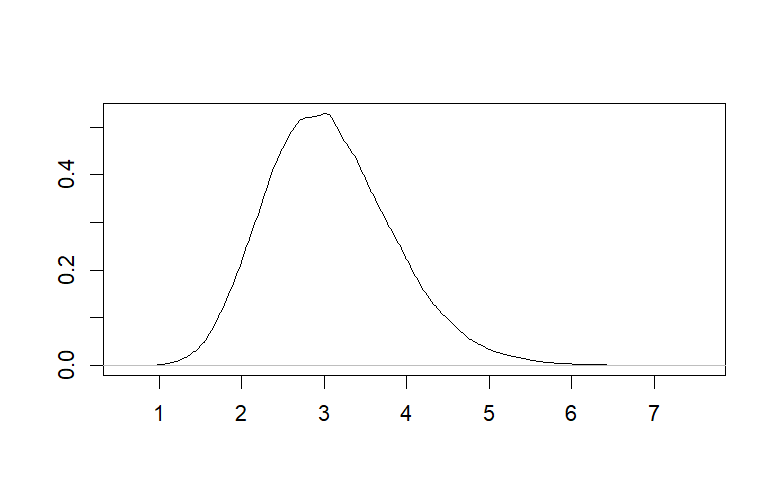
\includegraphics[width=\linewidth]{rytgaard1990_alpha_density.png}
        \subcaption{\( \alpha \)}
    \end{minipage}%
    \hfill
    \begin{minipage}{0.45\textwidth}
        \centering
        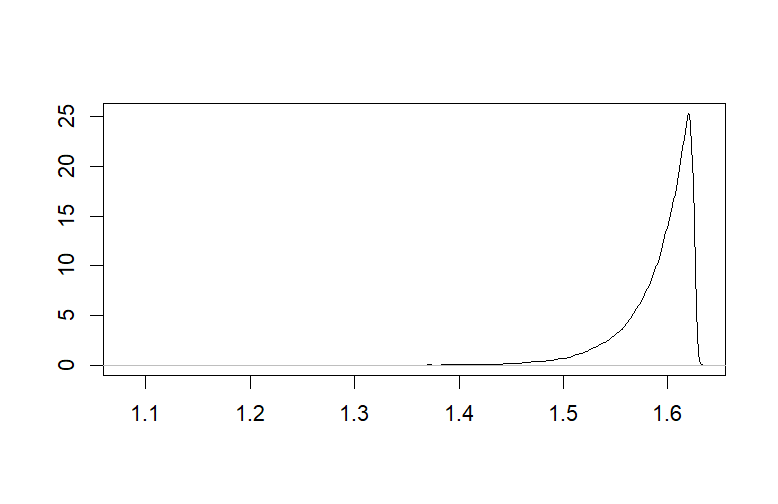
\includegraphics[width=\linewidth]{rytgaard1990_beta_density.png}
        \subcaption{\( \beta \)}
    \end{minipage} \\
    
%    \vspace{0.5cm}
    
    \begin{minipage}{0.45\textwidth}
        \centering
        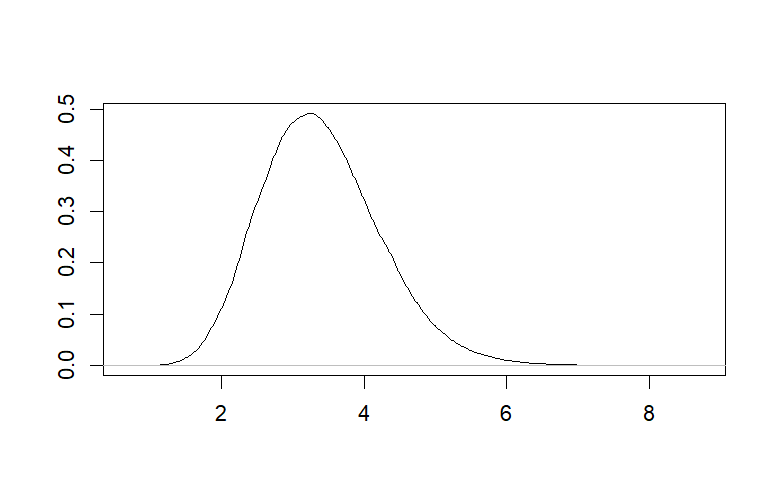
\includegraphics[width=\linewidth]{rytgaard1990_theta_density.png}
        \subcaption{\( \theta \)}
    \end{minipage}%
    \hfill
    \begin{minipage}{0.45\textwidth}
        \centering
        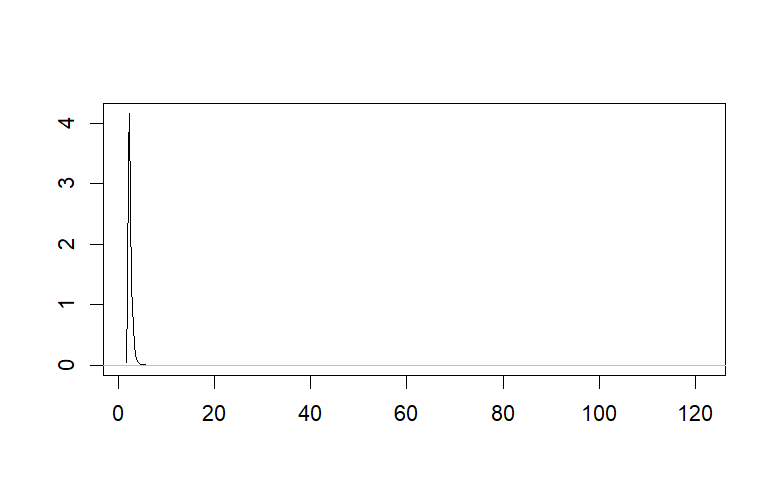
\includegraphics[width=\linewidth]{rytgaard1990_E_y_density.png}
        \subcaption{\( E[y] \)}
    \end{minipage}
    
    \caption{Posterior Densities}
    \label{fig:1}
\end{figure}

The posterior means of \( \alpha \) and \( \beta \) were used as parameters of the Pareto distribution, and the corresponding cumulative distribution function (CDF) was plotted against the empirical cumulative data (\( y_{i,t} \)). Similarly, the posterior mean of \( \theta \) was used as the parameter of the Poisson distribution, and its CDF was plotted against the empirical cumulative data (\( n_t \)).

\begin{figure}[!ht]
    \centering
    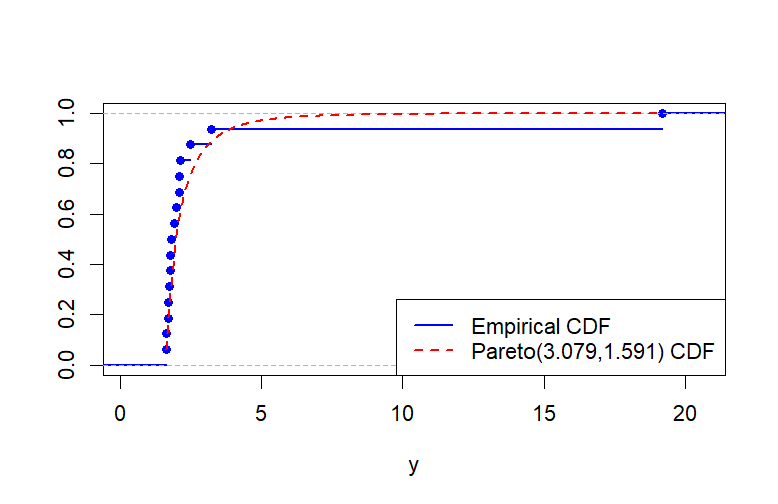
\includegraphics[width=0.8\textwidth]{empirical_vs_pareto.png}
    \caption{Empirical vs.\ Fitted Pareto CDF}
    \label{fig:2}
\end{figure}

\begin{figure}[!ht]
    \centering
    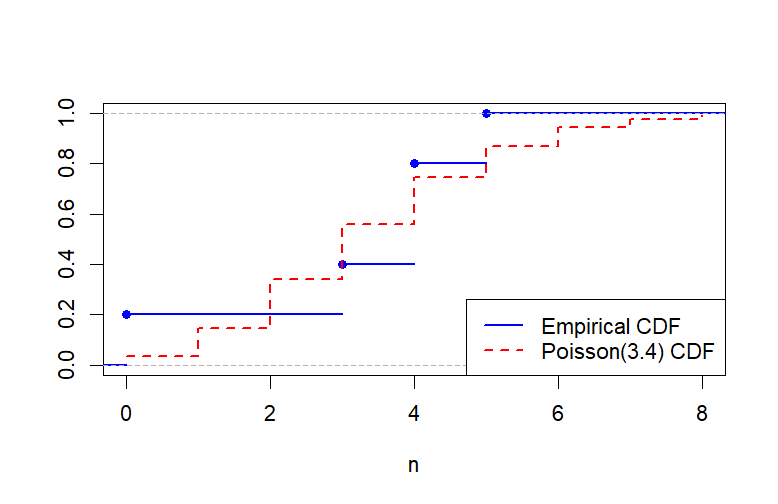
\includegraphics[width=0.8\textwidth]{empirical_vs_poisson.png}
    \caption{Empirical vs.\ Fitted Poisson CDF}
    \label{fig:3}
\end{figure}

The Pareto\((3.079,\,1.591)\) distribution provides a close fit to the empirical data. The Poisson\((3.4)\) distribution also fits the observed frequencies quite well.

Throughout all computations, a burn-in period of 20{,}000 iterations was applied, with only samples from iterations 20{,}001 to 50{,}000 retained for analysis. This approach follows the assumptions made by Dudley. However, it is essential to verify that the chains have indeed converged to a stationary distribution after discarding the initial samples. The first method of assessment involves visual inspection. Figure~\ref{fig:4} presents trace plots for all three parameters, showing the sampled values across iterations. These plots indicate good mixing, suggesting that the chains have converged.

\begin{figure}[!ht]
    \centering
    \begin{subfigure}{0.45\textwidth}
        \centering
        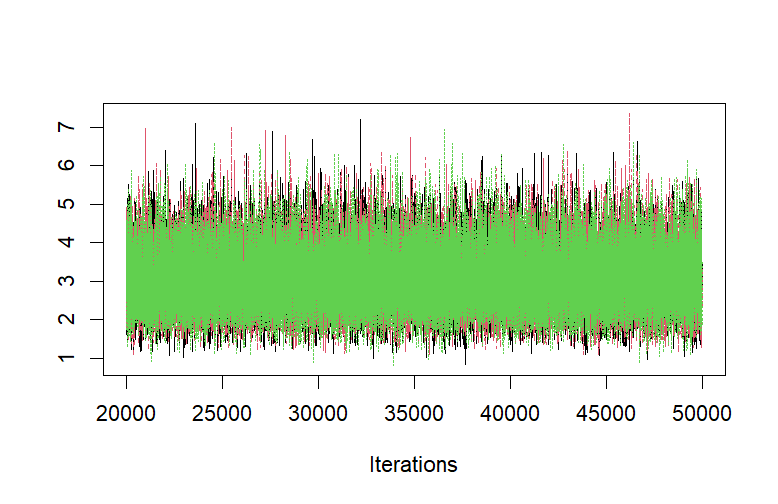
\includegraphics[width=\textwidth]{rytgaard1990_alpha_trace.png}
        \caption{Trace plot for \( \alpha \)}
    \end{subfigure}
    \hfill
    \begin{subfigure}{0.45\textwidth}
        \centering
        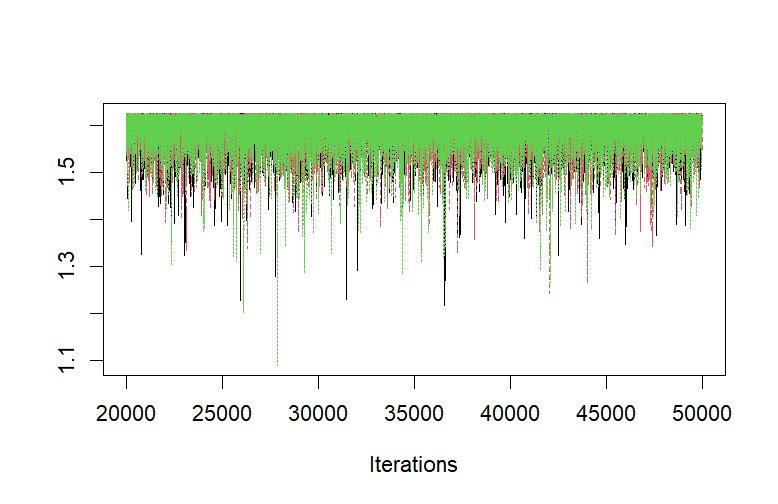
\includegraphics[width=\textwidth]{rytgaard1990_beta_trace.png}
        \caption{Trace plot for \( \beta \)}
    \end{subfigure}

    \vspace{1em}

    \begin{subfigure}{0.45\textwidth}
        \centering
        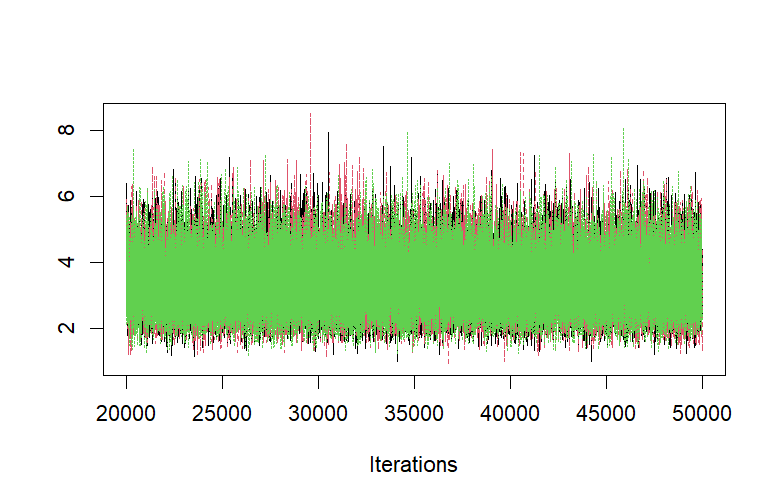
\includegraphics[width=\textwidth]{rytgaard1990_theta_trace.png}
        \caption{Trace plot for \( \theta \)}
    \end{subfigure}

    \caption{Trace Plots of Model Parameters}
    \label{fig:4}
\end{figure}

The convergence of the chains was also assessed using the Gelman--Rubin diagnostic. The diagnostic was applied to the post-burn-in iterations (20,001–50,000), and the results are summarized in Table~\ref{tab:psrf}.

\begin{table}[!ht]
\centering
\footnotesize
\caption{Potential Scale Reduction Factors (Gelman--Rubin Diagnostic)}
\label{tab:psrf}
\begin{tabular}{
  >{\raggedright\arraybackslash}p{\widthof{\textbf{Multivariate PSRF}}}
  *{2}{S[table-format=1.2]}
}
\hline
\textbf{Parameter} & \textbf{Point Estimate} & \textbf{Upper C.I.} \\
\hline
\( \alpha \) & 1.00 & 1.00 \\
\( \beta \)  & 1.00 & 1.01 \\
\( \theta \) & 1.00 & 1.00 \\
\hline
\textbf{Multivariate PSRF} & \multicolumn{2}{c}{1.00} \\
\hline
\end{tabular}
\end{table}

The results indicate that the chains have likely converged for all parameters, both individually and jointly.



\end{document}